%++++++++++++++++++++++++++++++++++++++++
% Don't modify this section unless you know what you're doing!
\documentclass{newseye_del}

\usepackage[utf8]{inputenc}


\usepackage[backend=biber, sorting=none]{biblatex}
\usepackage{csquotes}
\usepackage[english]{babel}

\usepackage{acronym}

\addbibresource{references.bib}


%+++++++++++++++++++++++++++++++++++++++++++++
%%%% All details should be filled in here %%%%
% Deliverable number:
\dnum{10.1}
% Deliverable full title
% (as in the description of the action -
% if needed, you may use a subtitle for better printing on the title page)
\title{Deliverable Template}
\subtit{}
% Deliverable short title
\shorttitle{Del. Templ.}
% Document identifier -
% please refer to the instructions of the quality management deliverable,
% annex A at https://drive.google.com/open?id=1Kgrj2NhfV8CiUIvwVncivTOVAyXn-oWK
% format = NewsEye-Tmm-Dnn-DeliverableShortName-status-vn.n.Extension
\docid{NewsEye-T101-D101-DelTempl-Submitted-v1.1.pdf}
% Lead partner
\resp{UH-CS}
% Report version
% please refer to the instructions of the quality management deliverable, annex A
\version{1.1}
% Date of completion of this version
\newdate{versiondate}{26}{2}{2019}
% Due date of deliverable
\newdate{duedate}{26}{3}{2020}
% Project month in which the deliverable is due
\duemonth{6}
% Dissemination level: PU, PP, RE or CO (see title page)
\distribution{CO}
% Deliverable type
\type{Template}
% Deliverable status, exactly one these options: Draft, Final or Submitted
\stat{Final}
% Author and co-authors, please put affiliation in parentheses for all
\mainauthor{Antoine Doucet (ULR)}
\coauthor{Mark Granroth-Wilding (UH-CS)}
% Reviewers
\intrew{Reviewer name (ULR)}
%+++++++++++++++++++++++++++++++++++++++++++++



\begin{document}

\titlepage

The NewsEye Consortium partner responsible for this deliverable has
addressed all comments received, making changes as necessary.
Changes to this document are detailed in the change log table below.

\vspace{10pt}
\textbf{Change Log}

\noindent
\begin{tabular}{ |p{2.5cm}|p{1.3cm}|p{4.2cm}|p{6.5cm}|  }
 \hline
 \rowcolor{lightgray} Date & Version & Editor & Summary of changes made\\
 \hline
  23/10/2018   & 1.0    & Antoine Doucet (ULR) & First template \\
 \hline
 	26/2/2019    & 1.1    & Mark Granroth-Wilding (UH-CS) & Tidied up and made easier to use \\
  \hline
\end{tabular}




\newpage
\section*{Executive summary}
\addcontentsline{toc}{section}{Executive Summary}

This report outlines the approach with which we will do stuff in the NewsEye
project. This is a short summary.

\newpage
\tableofcontents
\newpage


\section{Introduction}
\begin{abstract}
  Abstract here...
\end{abstract}

Short introduction here...


\section{The content}
The main content of the deliverable is organised in to sections.

\subsection{Subsection}
\label{sec:example subsection}

And subsections.

\paragraph{A paragraph title.}
You can also use \verb.\paragraph{}. for small divisions.

\section{Formatting}
Use standard \LaTeX formatting to write your document.

Format lists using \verb.\begin{itemize}..
\begin{itemize}
    \item Point 1
		\item Another point
\end{itemize}

Separate paragraphs using blank lines.

If you need to force a page break, use \verb.\newpage..

You can use footnotes using the \verb.\footnote{}. command\footnote{%
	Like this!
}.

\newpage

To include figures inline, using \verb.\begin{figure}[H]..
For example, the following chart provides an overview on the main components of the project:

\begin{figure}[H]
	\centering
	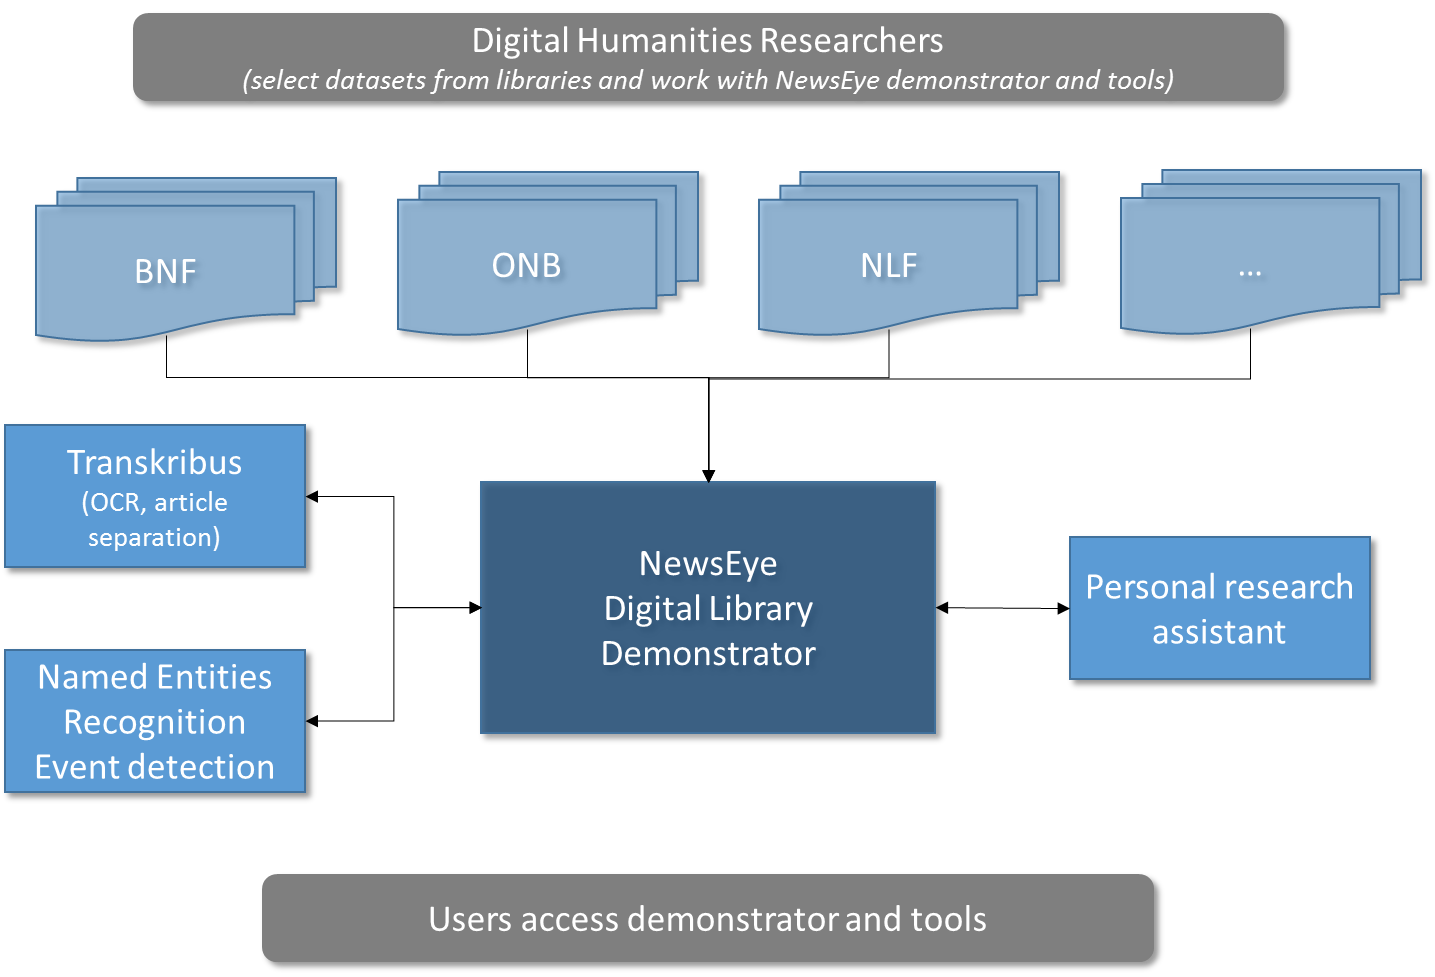
\includegraphics[width=0.7\textwidth]{overviewNewsEye.png}

	\caption{Overview of NewsEye}
	\label{fig:place}
\end{figure}



\section{References}
You can cite papers by adding them to \texttt{references.bib}
and then including the \verb.\cite{}. command to refere to them:
\cite{Crane2017}.

To update your bibliography, you need to run \texttt{pdflatex main},
then \texttt{biber main}, then \texttt{pdflatex main} again.


\href{https://www.newseye.eu/}{URLs} should be included using the \verb.\href{}{}. command.

Refer to sections within the document by placing a \verb.\label{myname}.
command at the start of the section, then using the \verb.\ref{myname}.
command to refer to it, as in the case of the
section~\ref{sec:example subsection}. Use the same method for referring
to figures, like fig.~\ref{fig:place}.



% Show the bibliography at the end
\newpage
\printbibliography

\end{document}
